
 \documentclass[hidelinks, a4paper,12pt,twoside]{report} % Please disbale the twocolumn later
% \usepackage{rpb_fin} %<- Contains all formatting stuff!
\usepackage{fin} %<- Contains all formatting stuff!
\usepackage[switch]{lineno} %\linenumbers % Place line on the side

\setcounter{tocdepth}{3} \brokenpenalty=10000 \tolerance=1 \emergencystretch=\maxdimen \hyphenpenalty=10000 \hbadness=10000
    \usepackage{cite} % 

% Start to enable during final version
		 %% Only enable during final print/
		\renewcommand{\cfttabfont}{Table } % Do not change, To allow in toc for text appear with Table 1.2 xxx
		\renewcommand{\cftfigfont}{Figure } % Do not change, To allow in toc for text appear with Figure 1.2 xxx: If disable, the toc text is without the word Figure
% End to enable during final version


% Start Package for table
			\usepackage{makecell}
			\newcolumntype{P}[1]{>{\centering\arraybackslash}p{#1}}
			\newcolumntype{M}[1]{>{\centering\arraybackslash}m{#1}}
			
			% From https://tex.stackexchange.com/questions/241892/two-figures-side-by-side-caption
			\usepackage{floatrow} 
			
			% From https://tex.stackexchange.com/questions/22751/how-to-force-table-caption-on-top
			% Forcing table caption on top
			\floatsetup[table]{capposition=top}
			
			
			% See: https://tex.stackexchange.com/questions/340433/formatting-table-with-siunitx-problem-with-special-format
			\usepackage{booktabs,siunitx} \sisetup{table-format=2.1}
%End Start Package for table

% Start graphic packing
			\usepackage{graphicx} 
			\newcommand{\plus}{\raisebox{.4\height}{\scalebox{.6}{+}}} 
			\graphicspath{ {./images/} }
		
			\usepackage[caption=false]{subfig}
% End graphic packing


% Start Math package
			\usepackage[cmex10]{amsmath} \DeclareMathOperator*{\argmax}{argmax}
			% \usepackage[classicReIm]{kpfonts}
			\usepackage{scalerel,amssymb} 
% End Math package


\def\msquare{\mathord{\scalerel*{\Box}{gX}}}
\def\msbigtriangledown{\mathord{\scalerel*{\bigtriangledown}{gX}}}
\def\mcirc{\mathord{\scalerel*{\bigcirc}{gX}}}


%% See: http://www.peteryu.ca/tutorials/publishing/latex_math_script_styles
\DeclareMathAlphabet{\mathpzc}{OT1}{pzc}{m}{it}
\usepackage{url}
\usepackage{hyperref}



% Shortcut

\usepackage{xspace} % Solve the spacing issue




\usepackage{setspace}% Modify the double/single spacing: For abstract > http://kb.mit.edu/confluence/pages/viewpage.action?pageId=3907092




\usepackage[open,openlevel=2]{bookmark}




\hyphenation{appli-cability}


\begin{document}


\pagestyle{plain}\cleardoublepage %To Add empty page and start on odd number (SOFTBOUND)%%

%\vspace{1 cm}
	
\raggedbottom 

\title{INOVATIVE: TO CREATE NEW MODULE FOR EFFECTIVENESS IN ADMINISTRATIVE STAFF WORKFLOW BY USING FULLY SISTEMIZE APPLICATION}
\author{YOUR NAME}
% \programfacul{INDUSTRIAL PHYSICS}
% \faculty{FACULTY OF SCIENCE AND NATURAL RESOURCES}


\degree{ BACHELOR OF SCIENCE WITH HONORS} % or \degree{Master of Science} 
\mainsupervisor{AP. Dr. Zoro}
% \cosupervisora{AP. Dr. Google}


\copyrightyear{\number\the\year} % or \copyrightyear{20xx}
\authoraddress{1234 Elm Street, Apt 567\\\hline Springfield, 98765\\\hline Any State, Malaysia\\\hline}


\beforepreface %dont change this


%-----------------------------------------------
\clearpage
\addcontentsline{toc}{section}{DEDICATION}
\prefacesection{Dedication}
\begin{center}
if you decide to dedicate your thesis to someone, it will be on a separate page.
\end{center}
%------------------------------------------------

%-----------------------------------------------
\prefacesection{Acknowledgements}
\renewcommand\listtablename{\normalsize\normalfont\centering\vspace*{-0.5in} ACKNOWLEDGEMENTS}
\begin{singlespace} 
	\setstretch{1.05}


It is good to thank here your supervisors and any sponsoring bodies, as well as any family,
friends, cats, dogs etc. that have been supportive during your time at University.
\end{singlespace}
%-----------------------------------------------
\iftablespage
\phantomsection
\addcontentsline{toc}{section}{ACKNOWLEDGEMENTS}% This adds the acknowledgement

%-----------------------------------------------
% \prefacesection{Abstract}
\prefacesection{\fontsize{14}{16}\fontfamily{phv}\selectfont \textbf{Abstract}}
\renewcommand\listtablename{\normalsize\normalfont\centering\vspace*{-0.5in} ABSTRACT}
\iftablespage
\phantomsection
\addcontentsline{toc}{section}{ABSTRACT}

According to the guidelines the abstract should not exceed 300 words. However, it is unlikely that anyone will be counting when you submit. If you still wish to do so, then better use
Emacs count-words command
%-----------------------------------------------


%-----------------------------------------------
\prefacesection{Abstrak}
\renewcommand\listtablename{\normalsize\normalfont\centering\vspace*{-0.5in} ABSTRACT}
\iftablespage
\phantomsection
\addcontentsline{toc}{section}{ABSTRAK}
\indent 
\begin{singlespace} 
if require Malay
\end{singlespace}

\clearpage
%-----------------------------------------------

% \newpage
% \thesiscopyrightpage %PLACING COPYRIGHT PAGE AFTER ABSTRAK (According to Aug 2012)
\afterpreface  %don't change this 
	\chapter{INTRODUCTION}
The introduction chapter of a thesis sets the stage for the entire research, providing the reader with essential background information, the context of the study, and a clear outline of the research objectives and significance. Each section within the introduction builds upon the previous one, gradually guiding the reader toward understanding the research problem and the purpose of the study. This section can be divided in multiple subsection to organize the information logically.

0\section{Background}

In this section, you aim to provide the reader with the foundational knowledge necessary to understand the broader context of your research. This includes explaining key concepts, relevant terminology.


\begin{figure}
	\centering
	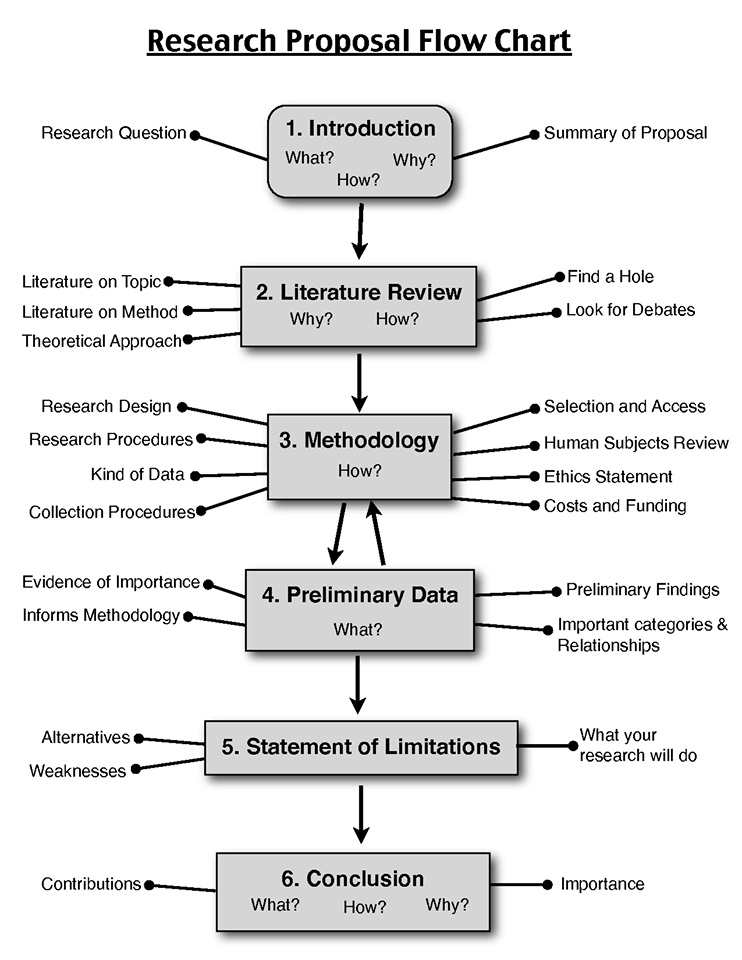
\includegraphics[width=15cm]{Writing research research proposal.png}
	\caption[Research Proposal Flow Chart]
	{The image is a flow chart titled "Research Proposal Flow Chart," designed to guide the development of a research proposal through six key stages: Introduction, Literature Review, Methodology, Preliminary Data, Statement of Limitations, and Conclusion. Each stage addresses specific questions like "What?", "Why?", and "How?", ensuring a comprehensive and structured approach. The chart outlines the progression from defining the research question and reviewing relevant literature, to detailing the methodology, presenting preliminary data, discussing limitations, and concluding with the significance of the research. This visual tool is essential for researchers in planning and articulating their study in a coherent and logical manner.. Figure adapted from \cite{Dorsett2010}.}
	\label{fig:ExxonSpreading}
\end{figure}
%


\subsection{Concept and Terminology Explanation}

In this subsection, you should broadly explain the key concepts and terminology that are central to your research. This will help ensure that readers who are not familiar with the topic can follow along.




\section{ Importance and Relevance} 
\label{SplitScheduleExplain}

In this subsection, explain why the topic is important and relevant. Include statistics, the impact of the topic on society, and any related government policies or initiatives. This helps to justify why your research is necessary and valuable.




\section{Motivation}

The motivation section of a thesis is crucial as it articulates the rationale behind the research, highlighting its importance and relevance. This section will help connects the background information with the research objectives by explaining why the study is necessary and what gaps it aims to fill. 

This section (and its subsection) builds a compelling case for the research by discussing the potential benefits and impact of the findings, thereby justifying the effort and resources invested in the study. The motivation section ensures that the reader understands the significance of the problem being addressed and the value that the proposed solutions can bring to the field.

You can give a brief overview or compact explaination from the literature review, what is there, but what is still missing. or the justification of why you insist of using some technique


\subsection{Some subsection to decompose your explaination}




\section{Problem Formulation}


\subsection{Research Gap}

The identified gap based on your literature review


\subsection{Problem Statement}

Based on the research gap, the following problems have been identified:

\begin{enumerate}
    \item \textbf{Definition of the Problem:} The problem statement clearly defines the issue that the research aims to address. It should describe the gap in knowledge, real-world challenges, or theoretical inconsistencies that necessitate investigation.

    \item \textbf{Relation to Hypotheses:} The problem statement serves as the foundation for formulating hypotheses. It outlines the research issue, while the hypotheses provide testable predictions based on this problem.

    \item \textbf{Best Practices for Writing a Problem Statement:}
    \begin{itemize}
        \item \textbf{Be clear and concise:} The problem statement should be straightforward, avoiding unnecessary jargon while effectively communicating the research issue.
        \item \textbf{Explain the research gap:} Clearly identify what is missing in existing research and why addressing this gap is important.
        \item \textbf{Define the scope:} Specify the boundaries of the problem, ensuring that it is neither too broad nor too narrow.
        \item \textbf{Highlight significance:} Explain why solving this problem is important, including its potential impact on the field, industry, or society.
        \item \textbf{Use evidence to support the problem:} Reference previous studies, statistics, or real-world examples to justify why the problem exists and why it requires investigation.
        \item \textbf{Ensure alignment with research objectives:} The problem statement should align with the study’s aims, ensuring consistency throughout the research process.
    \end{itemize}
\end{enumerate}


\section{Hypotheses of Study}
Based on the depicted problem statement, the following have been hypothesised:

\begin{enumerate}
    \item \textbf{Hypotheses:} A hypothesis is a testable statement or assumption that predicts the relationship between variables in a study. It serves as the foundation for research by providing a direction for investigation.

    \item \textbf{Relation to Problem Statement:} The problem statement defines the research issue and its significance, while hypotheses emerge from it as specific, testable propositions. The hypotheses offer potential explanations or solutions to the problem and guide data collection and analysis.

    \item \textbf{Best Practices for Writing Hypotheses:}
    \begin{itemize}
        \item \textbf{Be clear and specific:} A hypothesis should be precise and unambiguous, defining the variables and their expected relationship.
        \item \textbf{Ensure testability:} A good hypothesis should be measurable and testable using empirical methods.
        \item \textbf{Base it on existing knowledge:} Formulate hypotheses based on prior research, theories, or observations.
        \item \textbf{Use an "If-Then" structure (if applicable):} For causal relationships, use an "If X, then Y" format to establish a clear cause-and-effect relationship.
        \item \textbf{Make it falsifiable:} A hypothesis should be structured in a way that allows it to be proven false if the evidence contradicts it.
        \item \textbf{Keep it simple and focused:} Avoid overly complex hypotheses by keeping them concise and to the point.
    \end{itemize}
\end{enumerate}



\section{Research Question}

\begin{description}
    \item[RQ3] - Is there any significant correlation between social presence and course satisfaction among third-year Malaysian undergraduates undertaking a BL course in UMS?
    \item[RQ4] Is there any significant correlation between cognitive presence and course satisfaction among third-year Malaysian undergraduates undertaking a BL course in UMS?
    \item[RQ5] Which factor of teaching, social, and cognitive presence is dominant in determining course satisfaction among third-year Malaysian undergraduates undertaking a BL course in UMS?
\end{description}

\section{Study Objectives}



Based on the hypotheses, the following research objectives have been formulated:

\begin{enumerate}    
    \item  You may refer to online sources about SMART objectives, which define a goal that is specific, measurable, achievable, relevant, and time-bound.


       


    
\end{enumerate}



\section{Scope Of Work}

The scope of work for this thesis are:

\begin{enumerate}    


	
\end{enumerate}

\section{Organisation Of Thesis}
\label{ThesisOrganisation}


\noindent The organisation of this thesis is elaborated in the following:

Chapter 1 serves as an introduction, providing an overview of the study and emphasizing the importance of ... . You may eloborate more

Chapter 2 discusses relevant background information on.. . You may eloborate more

Chapter 3 details the development of the proposed method. You may eloborate more

Chapter 4 presents the experimental analysis and validation of the proposed . You may eloborate more

Chapter 5 summarizes key findings from each chapter, highlights the research contributions of this thesis in advancing.. You may eloborate more


The Chapter Appendix includes detailed explanations of the s. 
	% \chapter{LITERATURE REVIEW}

This chapter is composed of three main sections. The first section describes what a literature review is and explains its role in research. It highlights the importance of reviewing existing literature to understand the current state of knowledge on a topic and to build a foundation for further research. The second part of this chapter elaborates on the practical requirements to conduct a comprehensive literature review. It provides detailed steps on how to plan and execute the search for relevant literature. This includes choosing appropriate databases, using effective search strategies, and systematically analyzing and organizing the found information. Finally, the third section summarizes the key findings from the literature review and discusses their implications for the research field. It identifies gaps in current knowledge and suggests areas for future research. This section emphasizes how the literature review supports the research objectives and questions, providing a critical foundation for the subsequent chapters of the study.

\section{Introduction to Literature Review}
This section introduces the concept of a literature review and discusses its importance in research. A literature review serves as a critical summary of what the scientific community has published on a particular topic or subject. It provides an overview of current knowledge, allowing the researcher to position their own research within the existing literature.

\section{Conducting a Comprehensive Literature Review}
\subsection{Planning Your Literature Search}
Begin by defining clear objectives for your review. Determine the scope of your research and formulate research questions or hypotheses. Select databases and other sources relevant to your field of study. It is advisable to use a range of sources, including books, peer-reviewed journals, conference papers, and credible online resources.

\subsection{Searching for Relevant Literature}
Develop a search strategy using relevant keywords, phrases, and synonyms. Apply appropriate filters and Boolean operators (AND, OR, NOT) to refine your search results. Record your search strategies and results, which is essential for the reproducibility of your research.

\subsection{Screening and Selecting Literature}
Screen titles and abstracts for relevance to your research questions. Obtain and read full texts for selected sources. Use inclusion and exclusion criteria to systematically decide which articles to consider in your review.

\subsection{Analyzing and Synthesizing Information}
Organize the selected literature into thematic categories or according to methodological approaches. Analyze the findings and methodologies used in the literature to identify patterns, themes, and gaps in the research.

\subsection{Writing the Review}
Summarize the literature, linking it directly to your research questions and objectives. Discuss the significance of findings in relation to previous studies. Highlight any controversies, inconsistencies, and gaps in the literature. Present a critical analysis of the collected data, providing your interpretations and insights.




\begin{table}[h]
\centering
\caption{Comparison of Different Techniques}
\label{tab:technique_comparison}
\begin{tabular}{|c|m{6cm}|m{6cm}|}
\hline
\textbf{No.} & \textbf{Brief Note} & \textbf{Additional Details} \\ \hline
1 & Technique A: This technique is known for its speed and efficiency in processing large datasets. & Suitable for real-time applications. It can handle streaming data effectively but may require significant computational resources. \\ \hline
2 & Technique B: Often used for its high accuracy in classification tasks, especially in machine learning. & Requires extensive training data and is computationally expensive. It excels in scenarios where precision is critical. \\ \hline
3 & Technique C: Valued for its flexibility and adaptability across various domains. & While versatile, it may not provide the best performance in terms of speed or accuracy in specific applications. \\ \hline
\end{tabular}
\end{table}



\begin{table}[]
	\centering
	\caption{Reported results of the ternary sleepiness detection method in previous studies. }
	\label{tab:table3levelCompareOtherMinimal}
	\begin{tabular}{lllllll}
		\toprule[\heavyrulewidth] \toprule[\heavyrulewidth]
		No& Study   & Parameter(s) & Classifier   \\
		\midrule[\heavyrulewidth]
		1&\cite{Barua_2019} & 	EEG, EOG, CF& SVM \\
		2&\cite{Chai2019} & SWA & SVM \\
		3&\cite{Wang2016} & PERCLOS, SWA & 	MLO\\
		4&\cite{Zhao2015} & FE & NB \\
		5&\cite{Zhao2018} & FE & NB \\
		6&\cite{Zilin2017} & PERCLOS, EM & 	ANN\\
		7&\cite{Picot_2012} & 		EEG, EOG & 		CDR \\
		\hline	
	\end{tabular}
\end{table}

\section{Research Gap}

In the research gap section, it's important to find areas where questions still need answers or where current theories and methods don't fully solve the problems. This involves combining knowledge from previous studies you've reviewed, critically looking at their findings and methods, and spotting areas that haven't been fully explored yet. Doing this should help you see where you can make important improvements in the field, suggest new ways of researching, or address complex issues that haven't been dealt with thoroughly in past research.

\section{Chapter Summary}

A chapter summary in the literature review section is a brief overview of the key points covered in that chapter. It helps to consolidate the main findings, theories, and discussions presented. In this summary, you should clearly outline the most important ideas and how they relate to your research topic. This includes summarizing the debates, methodologies, and conclusions from various sources you've studied. The purpose of this summary is to give a clear and concise recap that helps readers understand the background and context of your study, and to set the stage for presenting the research gaps and questions your study aims to address.
 
	% % Updated 210719: 1932
\chapter{METHODOLOGY}

This chapter is composed of five main sections. Section 3.1 presents an overview of the proposed methodology, including a detailed flowchart of the experimental protocol. This flowchart visually outlines each step of the research process, from initial data collection to final analysis, providing a clear, step-by-step guide to how the research will be conducted. It also helps in illustrating the sequence of experimental procedures and how different phases of the study are interconnected. Section 3.2 discusses the criteria and procedures for selecting participants or data sources. It explains the sampling strategies, inclusion and exclusion criteria, and the methods employed to ensure a representative sample, enhancing the validity of the research findings. Section 3.3 describes the data collection methods used in the study. This section elaborates on each technique employed, such as surveys, interviews, or observations, and justifies their use in effectively gathering the necessary data. Section 3.4 outlines the data analysis procedures. It details the analytical techniques and tools used to interpret the data, whether involving statistical analysis for quantitative data or thematic analysis for qualitative data. Finally, Section 3.5 covers the ethical considerations of the research. It includes details on how informed consent was obtained, the steps taken to ensure the confidentiality and anonymity of participants, and the handling of any potential ethical issues throughout the study.


% This chapter is composed of five main sections. Section \ref{OverviewMethod} present an overview about the approach taken in this thesis in developing the SDS.
% Section \ref{BN_Variables}  presents a detailed account of the derivation of the sleepiness indicator that will be used as input into the machine learning.  
% %The first part present the approach to improve the subjective sleepiness estimation by using the combination of KDE and LR technique. The mathematical background of KDE and LR test is explained in detail. 
% Next, Section \ref{TechniqueBN} presents the framework of the proposed SDS. 
% Then, Section \ref{WorkaroundMissingKss} depicts the approach adopted to minimise the dependecy between the variable embedded in the proposed system as well as to increase the prediction horizon.
% Lastly, the section \ref{ComparativeStudy} explains in detail the criteria for validation metric, the types of validation, and the considerations taken in selecting evaluation metric.

\section{Overview Of The Proposed Methodology}

% \label{OverviewMethod}
%  \begin{figure}
% 	\centering
% 	\includegraphics[width=1\linewidth]{GeneralFlowChart}
% 	\caption[Flowchart of the experimental protocol]
% 	{Flowchart of the experimental protocol.}
% 	\label{Fig: GeneralFlowChart}
% \end{figure}


This chapter presents the complete methodology for the fulfillment of the research objectives formulated in Chapter 1. Section 3.1 details the design methodology chosen to achieve these objectives, as illustrated in Figure 2.1. This figure provides a visual flowchart of the experimental protocol, which maps out each step in the research process, from initial hypothesis formulation to data collection, analysis, and conclusion drawing. This systematic depiction ensures clarity in the research approach and facilitates a better understanding of how each phase interlinks and contributes to the overall study goals.



\subsection{Research Design}
This subsection should describe the overall framework of the study, whether it is experimental, correlational, or descriptive, and explain the rationale behind the chosen design.

\subsection{Participants}
\subsubsection{Sampling Strategy}
Detail how participants were selected, including the sampling methods and any demographic characteristics of interest.
\subsubsection{Inclusion and Exclusion Criteria}
Define the criteria for including or excluding participants in the study.

\subsection{Data Collection Methods}
\subsubsection{Quantitative Data}
Describe the instruments and tools used to collect numerical data, such as surveys or standardized tests.
\subsubsection{Qualitative Data}
Discuss the methods used to gather textual or observational data, like interviews or focus groups.

\subsection{Data Analysis}
\subsubsection{Statistical Analysis}
Outline the statistical techniques that will be applied to analyze the quantitative data.
\subsubsection{Thematic Analysis}
Describe how qualitative data will be analyzed, including any coding schemes or software used.

\subsection{Ethical Considerations}
Discuss how ethical issues were addressed, including participant consent and data privacy measures.

\section{Results} % Example of another chapter
\lipsum[1] % Filler text for demonstration




\section{Preparation For Comparative Study}
\label{ComparativeStudy}

\subsection{Evaluation Criteria }
\label{Data preparation}    

You may explain about the dataset here.



\subsection{Subject-wise Cross Validation for Performance Evaluation}    

you may explain how to validate



\subsection{Evaluation Metric}



\subsubsection{Box-Whisker Plot}

Box-whiskers plot and average \Fmeasure of the 24 selected subjects are reported in this study. Each box plot displays the median, the first and third quartile, as well as the minimum and maximum values. 
The notches around each median give a rough idea on the significantly varied medians: if the notches do not overlap, the medians differ at  5\% significance level. 
%An outlier (shown as red cross) is identified when a point exceeds the 25\superscripts{th} and 75\superscripts{th} percentiles. 
%The interval corresponds to approximately ±2.7$\sigma$ and 99.3\% coverage upon normally distributed data. The plotted whisker extends to the adjacent value, whereby the most extreme data value is not an outlier [60].
%% Please rephrase ^: From thesis: The Art of Heart Rate Variability Driver Fatigue Application


\subsubsection{Statistical Analyses}

The paired t-test was applied to ascertain the significant variance between the average \Fmeasure  of the proposed system and other techniques \cite{Demsar_2006}. The presence of outlier was determined by inspecting the boxplot for a value exceeding 1.5 box-length from the edge of the box in a boxplot. For each classifier performance, the normal distribution of the \Fmeasure  score was examined using Shapiro-Wilk’s test. As for \Fmeasure  performance that is not normally distributed, two t-tests were conducted by including and excluding the value of the outlier. The statistical significance was fixed at \LeqPointFive.


\section{Chapter Summary}
This chapter is composed up of five primary sections. The first section discussed the approach taken in this thesis in developing the system.


 
 %    % Updated 210719: 1932
\chapter{ RESULTS AND DISCUSSION}

This chapter presents the empirical outcomes and discusses in detail their significance to the field of study, as well as to the research community. When structuring the results and discussion chapter in an academic or research document, it's crucial to organize the content in a way that clearly presents your findings and interprets their implications. 


\section{Experimental Result}



\subsection{Presentation of Quantitative Data}
Describe and present the findings from the quantitative data through tables, graphs, and statistical analyses. Discuss significant trends or patterns observed in the data.




\subsection{Discussion Of The Results}

Discuss the implications of the results in the context of the existing literature or theories presented in earlier chapters. Interpret what the findings mean for the broader field of study.
Explicitly address how the results relate to each research question or hypothesis stated in the introduction. Discuss whether the findings support or refute the hypotheses.




\section{Qualitative Comparison With Other Studies}

In some cases, you may want to conduct Qualitative Comparison With Other Studies. In this case, you can consider to make a comparison table

\begin{table}[h]
	\centering
	\caption{Comparison of Various Industrial Physics Studies}
	\label{tab:industrialPhysicsCompare}
	\begin{tabular}{lll}
		\toprule[\heavyrulewidth] \toprule[\heavyrulewidth]
		Study & Parameter(s) & Acc (\%)  \\
		\midrule[\heavyrulewidth]
		\cite{Smith2020} & 
		Temperature, Pressure & 
		82.3\\

		\cite{Johnson2019} & 
		Velocity, Turbulence & 
		75.6\\

		\cite{Lee2018} & 
		Power Usage, Operational Hours & 
		89.1\\

		\cite{Kumar2017} & 
		Collision Energy, Particle Type & 
		91.4\\

		\cite{Chen2016} & 
		Frequency, Amplitude & 
		88.7\\

		\cite{Garcia2015} & 
		Chip Thickness, Impurity Levels & 
		84.9\\

		\cite{Morales2014} & 
		Solar Irradiance, Temperature & 
		79.3\\
		
		Proposed Method & 
		Microstructure Analysis, Load & 
		92.5\\ 
		\bottomrule[\heavyrulewidth]
	\end{tabular}
\end{table}






\section{Chapter Summary}

This chapter presents the findings and discussions related to the research questions outlined in the introduction. Initially, it systematically details the results obtained from both quantitative and qualitative analyses, using statistical data, graphical representations, and thematic interpretations to illustrate the key outcomes. Subsequently, the discussion section interprets these results in the context of existing literature, offering a comprehensive analysis of how the findings contribute to the broader field of study.

The chapter addresses each research question thoroughly, identifying whether the evidence supports or challenges the initial hypotheses. It also critically examines the limitations of the study's methodology and the impact these may have on the results. Furthermore, it explores the implications of the findings for future research and practical applications, suggesting directions for further studies and potential improvements in practice. The chapter concludes by summarizing the main findings and their significance, reinforcing the contribution of the study to the existing body of knowledge.
 
	% % Updated 210719: 1932
\chapter{CONCLUSION AND FUTURE DIRECTION}
\label{ch6}

\section{Overview}
This initial section provides a brief introduction to the concluding chapter. It sets the stage for summarizing the research findings, discussing their implications, and suggesting directions for future work. This overview should serve as a transition from the detailed analysis provided in the previous chapters to the summarization and forward-looking aspects of this final chapter.



\section{Conclusion Of The Study}

This section aims to clearly summarize the main results of your research and bring together your important findings into a final overview. It starts by briefly restating the main outcomes of the study, including a short explanation of the data analysis and results. Then, it focuses on the most important results and data points that directly address the research questions or hypotheses. It also discusses how these key findings are either similar to or different from the ideas and existing research that were mentioned earlier in your work. This helps to show how your results fit into the larger field of study.


\section{Contributions Of The Study}

This section outlines the unique contributions your study makes to its academic discipline or practical field. It starts by emphasizing any new methods you introduced or significant modifications you made to existing methods. Then, it discusses new insights or perspectives your research offers, highlighting how these enhance understanding within the field. Lastly, it describes how your results have expanded the existing body of knowledge, considering both theoretical and practical implications. This part of your study showcases the innovative aspects of your work and its impact on advancing knowledge.

\section{Future Work}

This section discusses the limitations of the current study and suggests directions for future research. It begins by openly addressing the shortcomings and constraints encountered during the research process, such as methodological limitations or data collection challenges. Next, it recommends specific areas where further investigation could yield additional insights, providing concrete suggestions for future researchers. Finally, it outlines strategies for overcoming the limitations identified in this study, suggesting the use of new methodologies, broader datasets, or alternative frameworks to enhance the robustness and scope of future research. This approach not only acknowledges the imperfections of the current study but also paves the way for subsequent advancements in the field. 
	% 




\section*{Appendix A: Dataset }


This appendix provides detailed information about the dataset used in the study. It includes descriptions of the ethical approvals obtained, the participants involved, and the experimental design employed.


\subsection*{Ethics Approval}
Before commencing the study, ethical approval was obtained from the Institutional Review Board (IRB) at [University Name]. The approval ensured that the research adhered to ethical guidelines, protecting the rights and welfare of all participants. The IRB approval number is [Approval Number], and the date of approval is [Approval Date]. All participants provided informed consent before participating in the study.

\subsection*{Participants}
The study involved a total of [Number] participants, recruited from [Source/Location]. The participants were selected based on specific inclusion and exclusion criteria to ensure a representative sample. The inclusion criteria included [list criteria], while the exclusion criteria included [list criteria]. The demographic breakdown of the participants is as follows: [Detail demographic information such as age, gender, education level, etc.].

\subsection*{Experimental Design}
The experimental design was structured to investigate [briefly describe the objective]. The study utilized a [describe the type of design, e.g., randomized controlled trial, between-subjects design, etc.]. Participants were randomly assigned to [number] groups: [describe the groups]. Each group underwent [describe the procedure or intervention]. Data were collected using [describe data collection methods, e.g., surveys, observations, measurements] at multiple time points: [list the time points]. The primary variables measured included [list primary variables]. The design ensured that the study was robust and capable of addressing the research questions effectively.



% 	\clearpage
% \addtocontents{toc}{\protect\setcounter{tocdepth}{0}}
% \addcontentsline{toc}{chapter}{LIST OF PUBLICATIONS}
% \chapter*{\normalsize \normalfont \vspace{-0.5in}\centering {LIST OF PUBLICATIONS}}

%\chapter*{\normalsize \normalfont \vspace{-0.5in}\centering {JOURNAL ARTICLES}}

%\section*{Journal articles}
% \begin{itemize}
% 	\item[\textbf{1.}] R. P. Balandong, T. T. Bong, M. Short, and M. N. Saad, 
% 	"Maritime Shift Workers Sleepiness Detection System With Multi-Modality Cues," 
% 	\textit{IEEE Access}, vol. 7, December. 2019.  \textbf{(Impact Factor: 4.098)}
	
% 	\item[\textbf{2.}] R. P. Balandong, R. F. Ahmad, M. N. Saad, and A. S. Malik, 
% 	"A Review on EEG-Based Automatic Sleepiness Detection Systems for Driver,"
% 	\textit{IEEE Access}, 
% 	vol. 6, May. 2017. 
% 	\textbf{(Impact Factor: 3.557)}	
% \end{itemize}


% \clearpage

% \begin{singlespace} 
% 	\setstretch{0.1}
% 	\smallskip
% 		\bibliographystyle{IEEEtran}
% 		\bibliography{BibThesis}
% \end{singlespace}


% \clearpage
% \addtocontents{toc}{\protect\setcounter{tocdepth}{0}}
% \addcontentsline{toc}{chapter}{APPENDICES}\label{appendix}
% \chapter*{\normalsize \normalfont \vspace{-0.5in}\centering {APPENDICES}}
% %\section*{test}
% \include{chap7}


	
\end{document} 


